\documentclass[a4paper,11pt]{article}
\input{/home/tof/Documents/Cozy/latex-include/preambule_lua.tex}
\newcommand{\showprof}{show them}  % comment this line if you don't want to see todo environment
\fancyhead[L]{Sécurité sur le web}
\newdate{madate}{10}{09}{2020}
%\fancyhead[R]{\displaydate{madate}} %\today
\fancyhead[R]{Seconde - SNT}
%\fancyhead[R]{Première - NSI}
%\fancyhead[R]{Terminale - NSI}
\fancyfoot[L]{~\\Christophe Viroulaud}
\AtEndDocument{\label{lastpage}}
\fancyfoot[C]{\textbf{Page \thepage/\pageref{lastpage}}}
\fancyfoot[R]{\includegraphics[width=2cm,align=t]{/home/tof/Documents/Cozy/latex-include/cc.png}}

\begin{document}
\begin{Form}
\section{Problématique}
La sécurité est une préoccupation importante sur le web. En effet, de nombreuses transactions financières se réalisent maintenant en ligne.
\begin{center}
\shadowbox{\parbox{12cm}{\centering Quelles sont les mesures mises en place pour sécuriser le web?}}
\end{center}
\section{Naviguer de manière sécurisée}
\subsection{Découvrir les notions}
\begin{activite}
Dans Pix, réaliser la compétence \emph{Sécuriser l'environnement numérique}.
\end{activite}
\subsection{Mode privé}
Depuis plusieurs années, tous les navigateurs proposent de naviguer en \emph{mode privé}. Ce mode de navigation peut porter à confusion. En effet, il ne garantit pas une navigation sécurisée, protégée des virus et autres pirates informatiques.
\begin{activite}
\begin{enumerate}
\item Ouvrir une fenêtre de navigation privée dans le navigateur. La page suivante \mbox{\url{https://tinyurl.com/yyqlbsq7}} propose un tutoriel pour la plupart des navigateurs courants.
\item Comment reconnaît-on que la page est en mode privé?
\item En effectuant une recherche, détailler l'action du mode privé.
\item Dans quels cas le mode privé peut-il alors être utile?
\item Le mode privé prévient-il lors du téléchargement accidentel d'un virus? Qui joue normalement ce rôle dans un ordinateur? 
\end{enumerate}
\end{activite}
\subsection{Page sécurisée}
\begin{activite}
\begin{enumerate}
\item Se rendre sur le site \mbox{\url{https://cviroulaud.github.io/}}.
\item Ce site est-il sécurisé? Comment le sait-on?
\item Quel organisme a délivré le certificat de sécurité pour ce site? 
\end{enumerate}
\end{activite}
\noindent La page web suivante \mbox{\url{https://tinyurl.com/y2xtode6}} détaille le fonctionnement d'une page web sécurisée.
\begin{activite}
Lire l'article de la page précédente et répondre aux questions:
\begin{enumerate}
\item Le site \emph{http://jay.info.free.fr} est-il sécurisé? Pour quelle raison?
\item À quel danger est-on confronté si on effectue une transaction sur ce site? 
\item Quel est le nom du projet de Google pour sécuriser le web? En quoi consiste-t-il?
\end{enumerate}
Les questions suivantes vont permettre de vérifier si ce site est sécurisé.
\begin{enumerate}[resume]
\item Entrer un identifiant et un mot de passe fictifs. \emph{Ne pas valider tout de suite.}
\\Choisir le raccourci en fonction du navigateur:
\item \textbf{Sur Firefox:}
\begin{enumerate}
\item  Cliquer sur \emph{Ctrl+Shift+E}, le panneau \emph{réseau} s'ouvre.
\item Dans la page web, valider le formulaire.
\item Ouvrir la ligne \emph{POST}.
\begin{center}
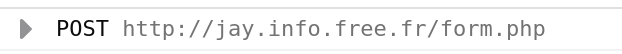
\includegraphics[width=7cm]{ressources/post-ff.png}
\end{center}
\item Dans \emph{Requêtes}, retrouver alors les informations transmises.
\end{enumerate}
\item \textbf{Sur Chrome:}
\begin{enumerate}
\item  Cliquer sur \emph{Ctrl+Shift+I}, un panneau s'ouvre.
\item Choisir \emph{Réseau} ou \emph{Network}.
\item Dans la page web, valider le formulaire.
\item Cliquer sur \emph{form.php}.
\begin{center}
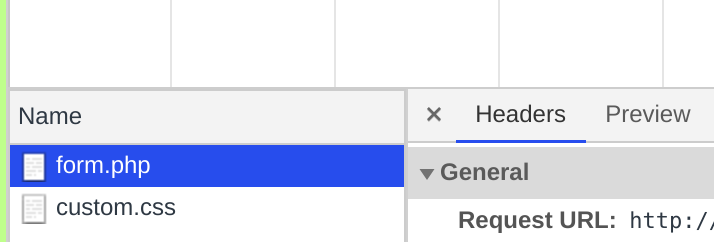
\includegraphics[width=6.5cm]{ressources/post-chrome.png}
\end{center}
\item Dans \emph{Headers}, retrouver alors les informations transmises.
\end{enumerate}
\end{enumerate}
\end{activite}
\begin{aretenir}[]
Sur un site non sécurisé, les informations sont transmises \textbf{en clair} entre les pages. Il est alors possible d'intercepter les données facilement.
\end{aretenir}
\section{Mots de passe}
\begin{activite}
\begin{enumerate}
\item Lire l'article sur la page \mbox{\url{https://tinyurl.com/yxmuv36s}}
\item Quel est le mot de passe le plus populaire en 2020?
\item Que peut-on dire du niveau de sécurité des mots passes les plus utilisés?
\item Se rendre sur le site \mbox{\url{https://tinyurl.com/y9l3cs4m}}
\item Calculer la forces des mots de passe suivants:
\begin{itemize}
\item 12345678
\item ABUEODNORR
\item AQIU12N9
\item AsSoI904nU12
\item A\%2sIP9\#Bb
\end{itemize}
\end{enumerate}
\end{activite}
\begin{commentprof}
\begin{itemize}
\item 12345678 $\;\rightarrow\;$27
\item ABUEODNORR $\;\rightarrow\;$47
\item AQIU12N9$\;\rightarrow\;$32
\item AsSoI904nU12 $\;\rightarrow\;$68
\item A\%2sIP9\#Bb$\;\rightarrow\;$61
\end{itemize}
\end{commentprof}
\end{Form}
\end{document}